%%----------------------------------------------------------------------------
%% Onderzoekstechnieken: Aan de slag (intro)
%%----------------------------------------------------------------------------

\documentclass[aspectratio=169]{beamer}

%==============================================================================
% Aanloop
%==============================================================================

%---------- Vormgeving --------------------------------------------------------

\usetheme{hogent}

\usecolortheme{hgwhite} % witte achtergrond, zwarte tekst

\usepackage{graphicx,multicol}
\usepackage{comment,enumerate,hyperref}
\usepackage{amsmath,amsfonts,amssymb}
\usepackage[dutch]{babel}
\usepackage{multirow}
\usepackage{eurosym}
\usepackage{listings}
\usepackage{textcomp}
\usepackage{framed}
\usepackage{wrapfig}
\usepackage{booktabs}

%---------- Configuratie ------------------------------------------------------

\usetikzlibrary{arrows,shapes,backgrounds,positioning,shadows}

%---------- Commando-definities -----------------------------------------------

\newcommand{\tabitem}{~~\llap{\textbullet}~~}
\newcommand{\alertbox}[1]{%
  \begin{center}
    \colorbox{hgblue}{\textcolor{white}{\textbf{#1}}}
  \end{center}
}

%---------- Info over de presentatie ------------------------------------------

\title{Hst 1. Aan de slag}
\subtitle{Onderzoekstechnieken}
\author{Jens Buysse \and Wim {De Bruyn} \and Bert {Van Vreckem} \and Pieterjan Maenhaut}
\date{AJ 2020-2021}

%==============================================================================
% Inhoud presentatie
%==============================================================================

\begin{document}

\begin{frame}
  \maketitle
\end{frame}

\begin{frame}
  \frametitle{What's on the menu today?}
  
  \tableofcontents
\end{frame}

\section{Onderzoekstechnieken}

\begin{frame}
  \frametitle{Onderzoekstechnieken}
  
  \centering
  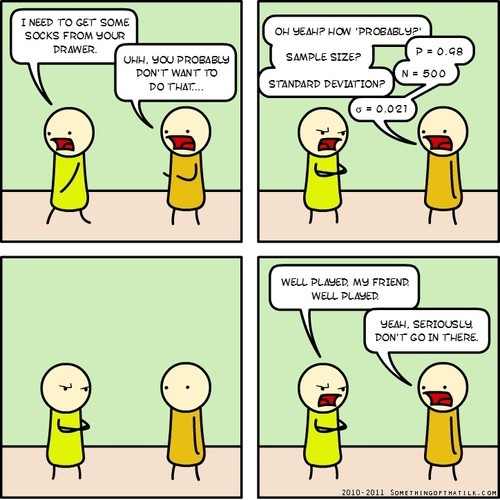
\includegraphics[height=.8\textheight]{intro-01.jpg}
\end{frame}

\begin{frame}
  \frametitle{Doel van deze cursus}
  
  \begin{itemize}
    \item Inleiding data science/statistiek
    \item Voorbereiding bachelorproef
  \end{itemize}
\end{frame}

\begin{frame}
  \frametitle{Leerdoelen en competenties}
  
  \begin{itemize}
    \item Kan begrippen, formules, stellingen en de uitwerking ervan uit de \textbf{beschrijvende en inductieve statistiek} benoemen en verklaren
    \item Kan formules, stellingen uit de beschrijvende en inductieve statistiek in onderzoeksvraagstukken correct \textbf{toepassen}
    \item Kan data \textbf{analyseren} met statistische software
    \item Kan een gestructureerd wetenschappelijk document \textbf{schrijven} en voorzien van referenties in \LaTeX{}
    \item Kan de \textbf{wetenschappelijke methode} vergelijken met niet-wetenschappelijke onderzoeksmethodes en daarbij voor- en nadelen opsommen 
  \end{itemize}
\end{frame}

\begin{frame}
  \frametitle{Hoe het niet moet}
  
  \centering
  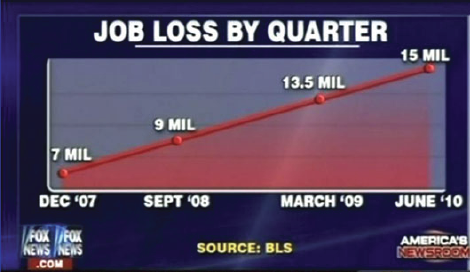
\includegraphics[height=.8\textheight]{intro-02.png}
\end{frame}

\begin{frame}
  \frametitle{Hoe het niet moet}
  
  \centering
  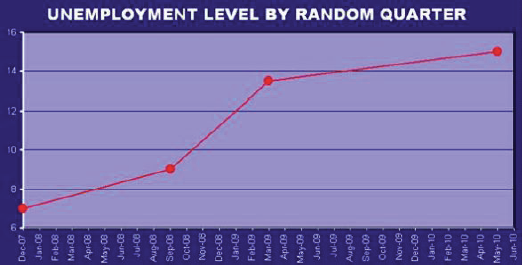
\includegraphics[height=.8\textheight]{intro-03.png}
\end{frame}

\begin{frame}
  \frametitle{Hoe het niet moet}
  
  \centering
  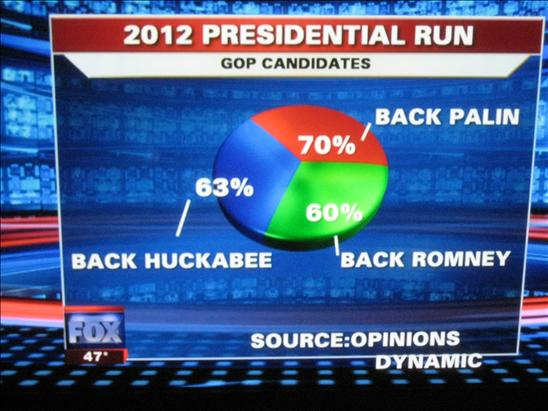
\includegraphics[height=.8\textheight]{intro-04.png}
\end{frame}

\begin{frame}
  \frametitle{Hoe het niet moet}
  
  \centering
  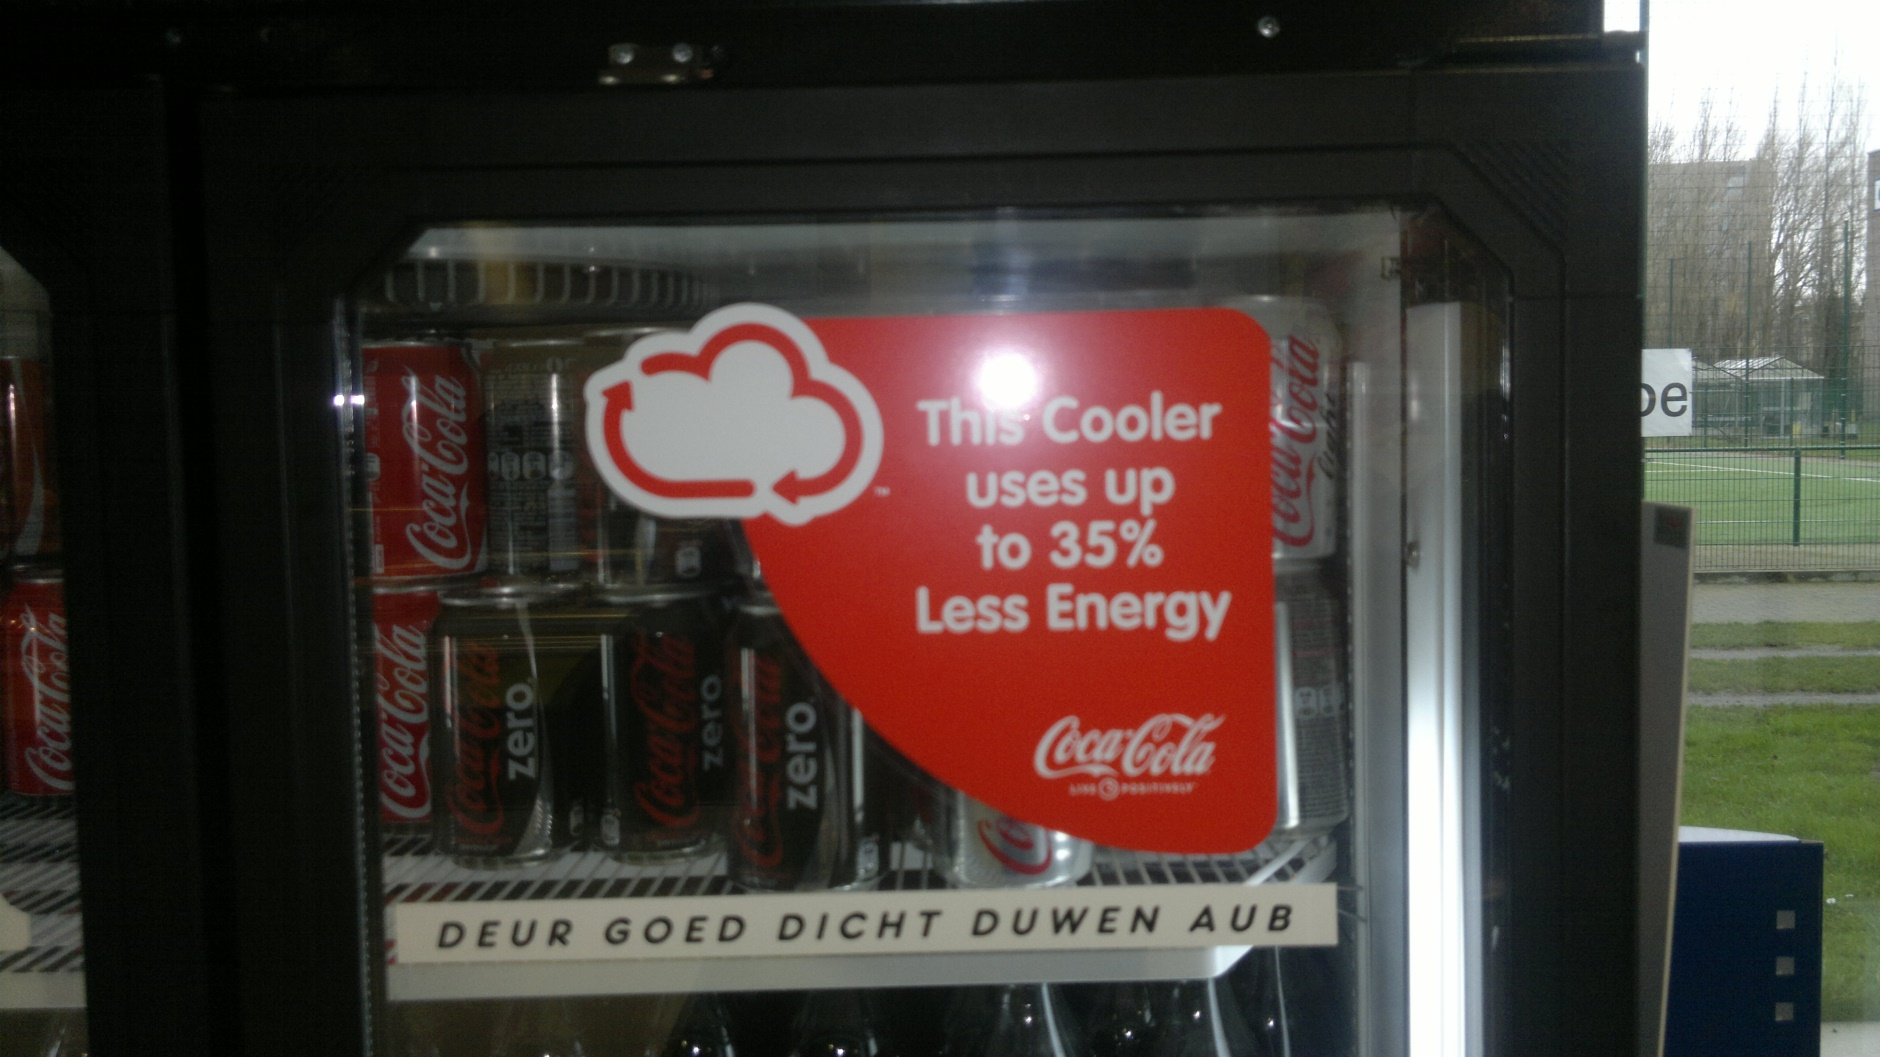
\includegraphics[height=.8\textheight]{intro-05.jpg}
\end{frame}

\begin{frame}
  \frametitle{Hoe het niet moet}
  
  \centering
  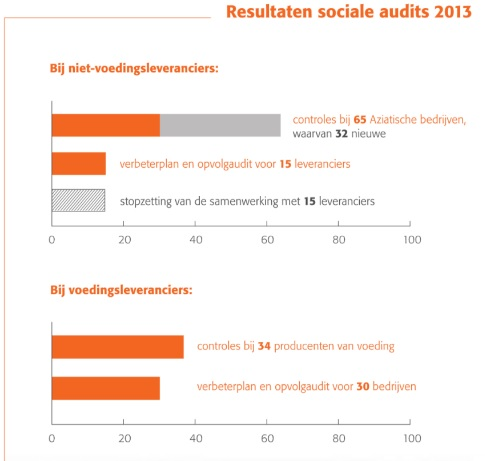
\includegraphics[height=.8\textheight]{intro-10.jpg}
\end{frame}

\begin{frame}
  \frametitle{Hoe het niet moet}
  
  \begin{figure}
    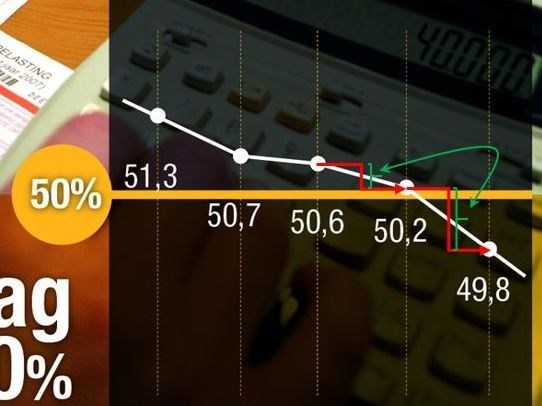
\includegraphics[height=.5\textheight]{intro-nva.jpg}
    \caption{Het overheidsbeslag is afgelopen jaar gedaald, maar niet zo spectaculair als een grafiek van de N-VA doet uitschijnen. Economieprofessor Tom Verbeke zag dat en wees N-VA met de vinger. ``Als een student dat soort truken toepast, zal hij zich serieus mogen verdedigen.''}
  \end{figure}
  
\end{frame}

\section{Studiewijzer}

\begin{frame}{Studiewijzer}
  Alle info over dit vak:
  
  \begin{itemize}
    \item Chamilo
    \item Studiefiche: via Chamilo of \url{https://www.hogent.be/studiefiches/}
    \item Studiewijzer: zie cursus, Hoofdstuk 1. \textit{Aan de slag}
  \end{itemize}
\end{frame}

\begin{frame}
  \frametitle{Leerinhoud}
  
  \begin{enumerate}
    \item Aan de slag
    \item Het onderzoeksproces
    \begin{itemize}
      \item De wetenschappelijke methode
      \item Basisconcepten, bv. variabelen, meetniveaus
      \item Steekproefonderzoek
    \end{itemize}
    \item Analyse van 1 variabele
    \begin{itemize}
      \item Centrum- en spreidingsmaten
      \item Visualisatie
    \end{itemize}
    \item De centrale limietstelling
    \begin{itemize}
      \item Kansverdeling van een steekproef
      \item De normale verdeling
      \item Betrouwbaarheidsintervallen
    \end{itemize}
  \end{enumerate}

\end{frame}

\begin{frame}
\frametitle{Leerinhoud (vervolg)}

  \begin{enumerate}
    \setcounter{enumi}{4}
    \item Toetsingsprocedures
    \begin{itemize}
      \item Hypothesetoetsen: basisbegrippen
      \item Kritiek gebied, overschrijdingskans
      \item $z$- en $t$-toets
    \end{itemize}
    \item Analyse van 2 variabelen
    \begin{itemize}
      \item Kruistabellen en $\chi^2$-toets, Cramér's $V$
      \item $t$-toets voor 2 steekproeven, Cohen's $d$
      \item Regressie-analyse, correlatie
      \item Visualisatie
    \end{itemize}
    \item Tijdreeksen
    \begin{itemize}
      \item Tijdreeksmodellen en voorspellen
      \item Voortschrijdend gemiddelde
      \item Exponentiële afvlakking, Holt-Winters
    \end{itemize}
  \end{enumerate}
\end{frame}

\begin{frame}
  \frametitle{Leermaterialen}

  \begin{itemize}
    \item Cursus (PDF via Chamilo, Github)
    \item Slides (PDF) ter ondersteuning
    \item Github repository met
    \begin{itemize}
      \item \LaTeX{} broncode cursus, slides
      \item R codevoorbeelden, tutorials
    \end{itemize}
  \end{itemize}    

\end{frame}

\begin{frame}
  \frametitle{Software}
  
  Instructies: zie cursus, hst 1.
  
  \begin{itemize}
    \item Git:
    \begin{itemize}
      \item Git client (CLI, GitKraken)
      \item Account op Github
    \end{itemize}
    \item {\LaTeX}:
    \begin{itemize}
      \item MikTeX/MacTeX/Texlive
      \item TexStudio
      \item JabRef (bibliografische databank)
    \end{itemize}
    \item Statistiek: R, RStudio Desktop
  \end{itemize}
  
  \centering
  Alle benodigde software is gratis/open source
\end{frame}

\begin{frame}
  \frametitle{Werkvormen}
  
  \begin{itemize}
    \item Hoorcollege (1u/w): theorie
    \item Werkcollege (2u/w):
    \begin{itemize}
      \item Uitdiepen kennis
      \item Oefeningen maken
      \item Leren werken met de software
    \end{itemize}
    \item Groepswerk, begeleide zelfstudie
    \begin{itemize}
      \item Doorloop onderzoeksproces
      \item Rapporteer over resultaten
    \end{itemize}
    \item Zelfstudie
    \begin{itemize}
      \item Leerstof bijhouden \& inoefenen!
    \end{itemize}
  \end{itemize}
\end{frame}

\begin{frame}
  \frametitle{Werk- en leeraanwijzingen}
  
  \begin{columns}
    \begin{column}{.8\textwidth}
        Onderzoekstechnieken wordt gezien als een moeilijk vak
      
      \begin{itemize}
        \item Kom naar de les
        \item Neem actief nota's!
        \item Werk ook buiten de contactmomenten
        \item Gebruik goede leertechnieken
        \item Stel vragen!
      \end{itemize}
      
      Zie studiewijzer
      
    \end{column}
  
    \begin{column}{.2\textwidth}
      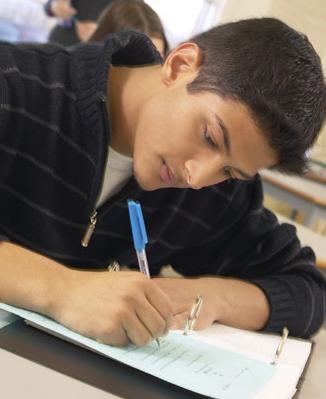
\includegraphics[height=2.5cm]{intro-06.jpg}
    \end{column}
  \end{columns}
  
\end{frame}

\begin{frame}
  \frametitle{Planning}
  \framesubtitle{Onder voorbehoud van verlofdagen, enz.}
  
  \centering
  \begin{tabular}{rl}
  	\toprule
  	\textbf{Week} & \textbf{Onderwerp}                \\
  	\midrule
  	            1 & Hst 1 -- Aan de slag              \\
  	              & Hst 2 -- Onderzoeksproces         \\
  	            2 & Hst 2 -- Onderzoeksproces         \\
  	            3 & Hst 3 -- Analyse van 1 variabele  \\
  	            4 & Hst 4 -- Centrale limietstelling  \\
  	            5 & Hst 5 -- Toetsingsprocedures      \\
  	            6 & Hst 5 -- Toetsingsprocedures      \\
  \end{tabular}
  
\end{frame}

\begin{frame}
  \frametitle{Planning}
  \framesubtitle{Onder voorbehoud van verlofdagen, enz.}
  
  \centering
  \begin{tabular}{rl}
  	\toprule
  	\textbf{Week} & \textbf{Onderwerp}                                           \\
  	\midrule
  	            7 & Hst 6 -- Analyse van 2 variabelen                            \\
  	              & \hspace{1.25cm} Kruistabellen, $\chi^2$ (toets)              \\
  	            8 & Hst 6 -- Analyse van 2 variabelen                            \\
  	              & \hspace{1.25cm} $t$-toets voor 2 steekproeven, effectgrootte \\
  	              & \textbf{Paasvakantie}                                        \\
  	            9 & Hst 6 -- Analyse van 2 variabelen                            \\
  	              & \hspace{1.25cm} Regressie-analyse, correlatie                \\
  	           10 & Hst 7 -- Tijdreeksen                                         \\
  	           11 & Voorbereiding bachelorproef                                  \\
  	           12 & Herhaling                                                    \\
  \end{tabular}
  
\end{frame}

\begin{frame}
  \frametitle{Evaluatie van het vak}

  \begin{columns}
    \begin{column}{.8\textwidth}
      \begin{itemize}
        \item Eerste examenkans
        \begin{itemize}
          \item Niet-periodegebonden evaluatie (NPE, groepswerk): 30\%
          \item Periodegebonden evaluatie (examen): 70\%
          \begin{itemize}
            \item 1u schriftelijk gesloten boek (theorie)
            \item 1u schriftelijk open boek met voorbereiding op eigen laptop (oefeningen)
          \end{itemize}
        \end{itemize}
        \item Tweede examenkans
        \begin{itemize}
          \item Niet-periodegebonden evaluatie: 30\%
          
          \textbf{overgenomen uit 1e zit}
          \item Periodegebonden evaluatie: 70\% (zoals 1e zit)
        \end{itemize}
      \end{itemize}
    \end{column}
    \begin{column}{.2\textwidth}
      
\includegraphics[height=3cm]{intro-07}
    \end{column}
  \end{columns}

\end{frame}

\begin{frame}
  \frametitle{NPE: Casus onderzoeksproces}
  
  \alertbox{Welke factoren beïnvloeden hoe goed je bent in wiskunde?}
  
  \begin{enumerate}
    \item Literatuuronderzoek
    \item Onderzoeksvraag afbakenen en vastleggen
    \item Onderzoeksgegevens verzamelen (enquête)
    \item Resultaten statistisch verantwoord analyseren
    \item Verslaggeving over het onderzoek
  \end{enumerate}
  
  Opdrachtbeschrijving op Chamilo, onder Opdrachten
\end{frame}

\end{document}